\section{Infinite Series} \label{S:7.2.Sequences}

\begin{goals}
\item What is an infinite series?
\item What is the $n$th partial sum of an infinite series?
\item How do we add up an infinite number of numbers? In other words, what does is mean for an infinite series of real numbers to converge?
\item What does is mean for an infinite series of real numbers to diverge?

\end{goals}

%-----------------------------------
% SUBSECTION INTRODUCTION
%-----------------------------------
\subsection*{Introduction}

Given the sequence $\{a_n\} = \{1/2^n\} = 1/2,\ 1/4,\ 1/8,\ \ldots$, consider the following sums:

$$\begin{array}{ccccc}
a_1				&=& 1/2					 &=& 1/2\\
a_1+a_2		&=& 1/2+1/4			 &=& 3/4\\
a_1+a_2+a_3 &=& 1/2+1/4+1/8  &=& 7/8\\
a_1+a_2+a_3+a_4 &=& 1/2+1/4+1/8+1/16 & =& 15/16
\end{array}$$
In general, we can show that $$a_1+a_2+a_3+\cdots +a_n = \frac{2^n-1}{2^n} = 1-\frac{1}{2^n}.$$
Let $S_n$ be the sum of the first $n$ terms of the sequence $\{1/2^n\}$. From the above, we see that $S_1=1/2$, $S_2 = 3/4$, etc. Our formula at the end shows that $S_n = 1-1/2^n$. 

Now consider the following limit: $\ds \lim_{n\to\infty}S_n = \lim_{n\to\infty}\big(1-1/2^n\big) = 1$. This limit can be interpreted as saying something amazing: \emph{the sum of \emph{all} the terms of the sequence $\{1/2^n\}$ is 1.} 


This example illustrates some interesting concepts that we explore in this section. We begin this exploration with some definitions.

\definition{Infinite Series, $n^\text{th}$ Partial Sums, Convergence, Divergence}  %definition
{Let $\{a_n\}$ be a sequence.
\begin{enumerate}
\item		The sum $\ds a_1 + a_2 + \cdots + a_n + \cdots =\sum_{n=1}^\infty a_n$ is an \textbf{infinite series} (or, simply \textbf{series}).
\item		Let $\ds S_n = a_1 + a_2 + \cdots + a_n = \sum_{i=1}^n a_i$; the sequence $\{S_n\}$ is the sequence of \textbf{$n^\text{th}$ partial sums} of $\{a_n\}$.
\item		If the sequence $\{S_n\}$ converges to $L$, we say the series $\ds \sum_{n=1}^\infty a_n$ \textbf{converges} to $L$, and we write $\ds \sum_{n=1}^\infty a_n = L$.
\item		If the sequence $\{S_n\}$ diverges, the series $\ds \sum_{n=1}^\infty a_n$ \textbf{diverges}.
\index{series!definition}\index{series!partial sums}\index{series!convergent}\index{series!divergent}\index{convergence!of series}\index{divergence!of series}
\end{enumerate}
}  %end definition


Using our new terminology, we can state that the series $\ds \sum_{n=1}^\infty 1/2^n$ converges, and $\ds \sum_{n=1}^\infty 1/2^n = 1.$

We will explore a variety of series in this section. We start with two series that diverge, showing how we might discern divergence.

\begin{marginfigure}[4cm] % MARGIN FIGURE
\subfloat[]{\margingraphics{figures/figseries1a}}

\subfloat[]{\margingraphics{figures/figseries1b}}

\subfloat[]{\margingraphics{figures/figseq1c}}
\caption{Scatter plots relating to Example \ref{eg:7.2.1}.} \label{F:eg:7.2.1}
\end{marginfigure}

\begin{example} \label{eg:7.2.1} % EXAMPLE
\begin{enumerate}
\item		Let $\{a_n\} = \{n^2\}$. Show $\ds \sum_{n=1}^\infty a_n$ diverges.
\item		Let $\{b_n\} = \{(-1)^{n+1}\}$. Show $\ds \sum_{n=1}^\infty b_n$ diverges.
\end{enumerate}

\solution
\begin{enumerate}
\item	Consider $S_n$, the $n^\text{th}$ partial sum.
\begin{align*} S_n &= a_1+a_2+a_3+\cdots+a_n \\		
						&= 1^2+2^2+3^2\cdots + n^2.
\intertext{By Theorem \ref{thm:summation}, this is}
						&= \frac{n(n+1)(2n+1)}{6}.
\end{align*}
Since $\ds \lim_{n\to\infty}S_n = \infty$, we conclude that the series $\ds \sum_{n=1}^\infty n^2$ diverges. It is instructive to write $\ds \sum_{n=1}^\infty n^2=\infty$ for this tells us \emph{how} the series diverges: it grows without bound.

A scatter plot of the sequences $\{a_n\}$ and $\{S_n\}$ is given in Figure \ref{F:eg:7.2.1}(a). The terms of $\{a_n\}$ are growing, so the terms of the partial sums $\{S_n\}$ are growing even faster, illustrating that the series diverges.


\item		Consider some of the partial sums $S_n$ of $\{b_n\}$:
\begin{align*}
S_1 &= 1\\
S_2 &= 0\\
S_3 &= 1\\
S_4 &= 0
\end{align*}
This pattern repeats; we find that $S_n = \left\{\begin{array}{cc} 1  & n\ \text{ is odd}\\
																																		0  & n\  \text{ is even}
																								\end{array}\right..$
As $\{S_n\}$ oscillates, repeating 1, 0, 1, 0, $\ldots$, we conclude that $\ds\lim_{n\to\infty}S_n$ does not exist, hence $\ds\sum_{n=1}^\infty (-1)^{n+1}$ diverges.		

A scatter plot of the sequence $\{b_n\}$ and the partial sums $\{S_n\}$ is given in Figure \ref{F:eg:7.2.1}(b). When $n$ is odd, $b_n = S_n$ so the marks for $b_n$ are drawn oversized to show they coincide.	
																					
\end{enumerate}
\end{example}

While it is important to recognize when a series diverges, we are generally more interested in the series that  converge. In this section we will demonstrate a few general techniques for determining convergence; later sections will delve deeper into this topic. First, the activity demonstrates an important series that has many applications.

\begin{activity} \label{A:7.2.1}  
  Warfarin is an anticoagulant that prevents blood clotting; often it is prescribed to stroke victims in order  to help ensure blood flow. The level of warfarin has to reach a certain concentration in the blood in order to be effective. 

Suppose warfarin is taken by a particular patient in a 5 mg dose each day. The drug is absorbed by the body and some is excreted from the system between doses. Assume that at the end of a 24 hour period, 8\% of the drug remains in the body. Let $Q(n)$ be the amount (in mg) of warfarin in the body before the $(n+1)$st dose of the drug is administered.

\ba
\item Explain why $Q(1) = 5 \times 0.08$ mg.

\item Explain why $Q(2) = (5+Q(1)) \times 0.08$ mg. Then show that 
\[Q(2) = (5 \times 0.08)\left(1+0.08\right) \text{ mg}.\]

\item Explain why $Q(3) = (5+Q(2)) \times 0.08$ mg. Then show that
\[Q(3) = (5 \times 0.08)\left(1+0.08+0.08^2\right) \text{ mg}.\]

\item Explain why $Q(4) = (5+Q(3)) \times 0.08$ mg. Then show that
\[Q(4) = (5 \times 0.08)\left(1+0.08+0.08^2+0.08^3\right) \text{ mg}.\]

\item There is a pattern that you should see emerging. Use this pattern to find a formula for $Q(n)$, where $n$ is an arbitrary positive integer.

\item Complete Table \ref{T:8.2_Warfarin} with values of $Q(n)$ for the provided $n$-values (reporting $Q(n)$ to 10 decimal places). What appears to be happening to the sequence $Q(n)$ as $n $ increases?
\begin{table}[ht]
\begin{center}
\renewcommand{\arraystretch}{1.5}
\begin{tabular}{c|c}
$Q(1)$   & $0.40$ \\
$Q(2)$   & \\
$Q(3)$   &  \\
$Q(4)$   &  \\
$Q(5)$   &  \\
$Q(6)$   &  \\
$Q(7)$   &  \\
$Q(8)$   &  \\
$Q(9)$   &  \\
$Q(10)$  &  \\
\end{tabular}
\caption{Values of $Q(n)$ for selected values of $n$}
\label{T:8.2_Warfarin}
\end{center}
\end{table}

%\begin{itemize}
%\item After the first dose is administered, the body will absorb the drug and retain 8\% of the dose. So
%\[Q(1) = 5 \times 0.08 \text{ mg}.\]
%\item After the second dose is administered, the body will absorb the drug and retain 8\% of the dose, plus what remained in the body after the second dose. So
%\[Q(2) = 5 \times 0.08 + \left(0.08 \times 5\right) \times 0.08 = (5 \times 0.08)\left(1+0.08\right) \text{ mg}.\]
%\item After the third dose is administered, the body will absorb the drug and retain 8\% of the dose, plus what remained in the body after the third dose. So
%\[Q(3) = 5 \times 0.08 + \left(0.08 \times 5\right) \left(1+0.08\right)\times 0.08 = (5 \times 0.08)\left(1+0.08+0.08^2\right) \text{ mg}.\]
%\item After the fourth dose is administered, the body will absorb the drug and retain 8\% of the dose, plus what remained in the body after the fourth dose. So
%\[Q(4) = 5 \times 0.08 + \left(0.08 \times 5\right) \left(1+0.08+0.08^2\right)\times 0.08 = (5 \times 0.08)\left(1+0.08+0.08^2+0.08^3\right) \text{ mg}.\]
%\end{itemize}


%A pattern seems to be emerging. It appears that after the $n$th dose is administered, the body will absorb the drug and retain 8\% of the dose, plus what remained in the body after the $n$th dose and so
%\begin{equation} \label{eq:8.2_part_sum}
%Q(n)=(5 \times 0.08)\left(1+0.08+0.08^2+0.08^3+ \cdots + 0.08^{n-1}\right) \text{ mg}.
%\end{equation}

%*** begin comment ***

%Table \ref{T:8.2_Warfarin} gives the values of $Q(n)$ for a few selected values (to 10 decimal places) of $n$:
%\begin{table}[ht]
%\begin{center}
%\renewcommand{\arraystretch}{1.5}
%\begin{tabular}{c|c}
%$Q(1)$   & $0.40$ \\
%$Q(2)$   & $0.432$ \\
%$Q(3)$   & $0.43456$ \\
%$Q(4)$   & $0.4347648$ \\
%$Q(5)$   & $0.434781184$ \\
%$Q(6)$   & $0.4347824948$ \\
%$Q(7)$   & $0.4347825996$ \\
%$Q(8)$   & $0.4347826080$ \\
%$Q(9)$   & $0.4347826088$ \\
%$Q(10)$  & $0.4347826088$ \\
%\end{tabular}
%\caption{Values of $Q(n)$ for selected values of $n$}
%\label{T:8.2_Warfarin_Sol}
%\end{center}
%\end{table}
%We can plot the data points $(n,Q(n))$ and visualize the long-term behavior as shown in Figure \ref{F:8.2.Warfarin}

%\begin{figure}[h]
%\begin{center}
%\resizebox{!}{1.5in}{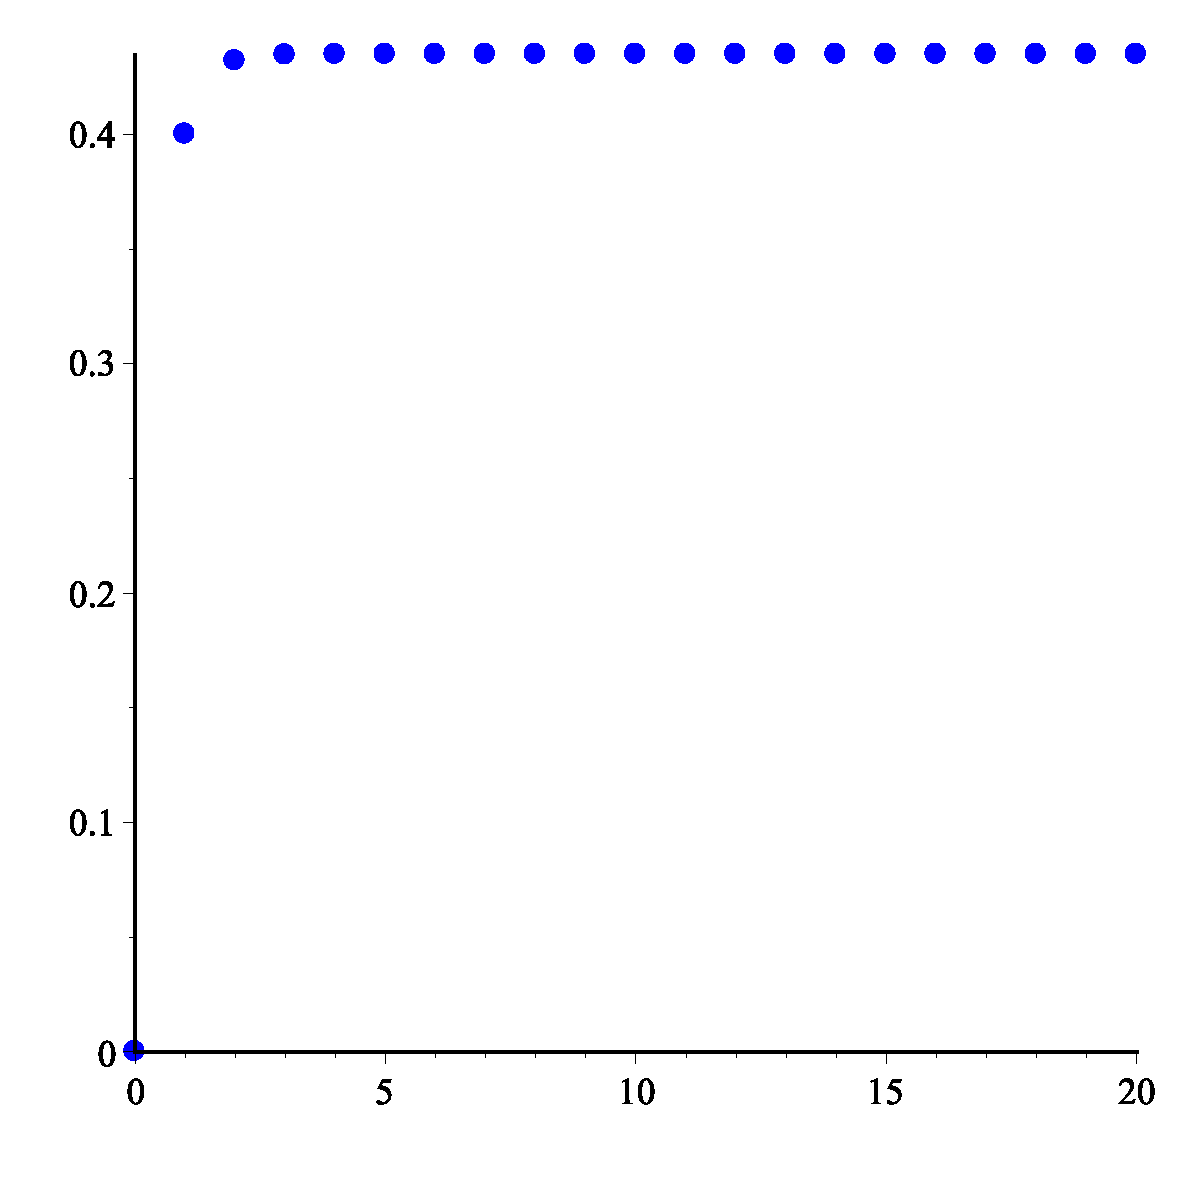
\includegraphics{figures/8_2_Warfarin.eps}}
%\caption{The points $(n, Q(n))$ for $n$ from 1 to 20}
%\label{F:8.2.Warfarin}
%\end{center}
%\end{figure}

%The data and the graph appears to indicate there is a long-term level of Warfarin that remains in the blood, or a limit to the sequence of values $Q(n)$ as $n$ goes to infinity. The data approximates this ling-term level, but with a little more work we can find the exact level of Warfarin in the blood.

%*** end comment ****


\ea
\end{activity}


\begin{smallhint}
\ba
	\item Small hints for each of the prompts above.
\ea
\end{smallhint}
\begin{bighint}
\ba
	\item Big hints for each of the prompts above.
\ea
\end{bighint}
\begin{activitySolution}
\ba
	\item Solutions for each of the prompts above.
\ea
\end{activitySolution}
\aftera % ACTIVITY


%-------------------------------
% SUBSECTION Geometric Series
%-------------------------------
\subsection*{Geometric Series} \index{geometric series}

In Activity \ref{A:7.2.1} we encountered the sum
\[(5 \times 0.08)\left(1+0.08+0.08^2+0.08^3+ \cdots + 0.08^{n-1}\right).\]
In order to evaluate the long-term level of Warfarin in the patient's system, we will want to fully understand the sum in this expression. This sum has the form
\begin{equation} \label{eq:7.2_part_sum_geometric_1}
a+ar+ar^2+ \cdots + ar^{n-1}
\end{equation}
where $a=5 \times 0.08$ and $r=0.08$. Such a sum is called a \emph{geometric sum}\index{geometric sum} with ratio $r$. When the sum has infinite terms it is called a \emph{geometric series}.

\definition{Geometric Series} %definition
{A \textbf{geometric series} is a series of the form 
$$\sum_{n=0}^\infty r^n = 1+r+r^2+r^3+\cdots+r^n+\cdots$$
Note that the index starts at $n=0$, not $n=1$.%
\index{series!geometric}\index{geometric series}
} %end definition

We started this section with a geometric series, although we dropped the first term of $1$. One reason geometric series are important is that they have nice convergence properties.

\concept{Convergence of Geometric Series}
{Consider the geometric series $\ds \sum_{n=0}^\infty r^n$.
\begin{enumerate}
\item		The $n^\text{th}$ partial sum is: $\ds S_n = \frac{1-r\,^{n+1}}{1-r}$.
\item		The series converges if, and only if, $|r| < 1$. When $|r|<1$, 
\index{series!geometric}\index{geometric series}\index{convergence!of geometric series}\index{divergence!of geometric series}
$$\sum_{n=0}^\infty r^n = \frac{1}{1-r}.$$
\end{enumerate}
}

\begin{activity} \label{A:7.2.2}  
Let $a$ and $r$ be real numbers (with $r \ne 0$) and let
\[S_n = a+ar+ar^2 + \cdots + ar^{n-1}.\]
In this activity we will find a shortcut formula for $S_n$ that does not involve a sum of $n$ terms.
\ba
\item Multiply $S_n$ by $r$. What does the resulting sum look like?


\item Subtract $rS_n$ from $S_n$ and explain why
\begin{equation} \label{eq:7.2.1_partial_geometric_sum}
S_n - rS_n = a - ar^n.
\end{equation}


\item Solve equation (\ref{eq:7.2.1_partial_geometric_sum}) for $S_n$ to find a simple formula for $S_n$ that does not involve adding $n$ terms.


\ea
\end{activity}

\begin{smallhint}
\ba
	\item Small hints for each of the prompts above.
\ea
\end{smallhint}
\begin{bighint}
\ba
	\item Big hints for each of the prompts above.
\ea
\end{bighint}
\begin{activitySolution}
\ba
	\item Note that
\[rS_n = ar+ar^2+ar^3 + \cdots + ar^n.\]
    \item When we subtract $rS_n$ from $S_n$ the middle terms all cancel and we are left with
\begin{align*}
S_n - rS_n &= \left(a+ar+ar^2 + \cdots + ar^{n-1}\right) - \left(ar+ar^2+ar^3 + \cdots + ar^n\right) \\
    &=a + (ar-ar) + \left(ar^2-ar^2\right) + \cdots + \left(ar^{n-1}-ar^{n-1}\right) - ar^n \\
    &= a - ar^n.
    \end{align*}
    \item Factoring $S_n$ from left hand side and dividing gives us a formula for $S_n$:
\begin{align*}
S_n(1-r) &= a - ar^n \\
S_n &= a\frac{1-r^n}{1-r}.
\end{align*}

\ea
\end{activitySolution}
\aftera %activity

According to the concept above, the series $\ds\sum_{n=0}^\infty \frac{1}{2^n} = 1+\frac12+\frac14+\cdots$ converges, and $\ds \sum_{n=0}^\infty \frac{1}{2^n} = \frac{1}{1-1/2} = 2.$ This concurs with our introductory example; while there we got a sum of 1, we skipped the first term of 1.

\begin{marginfigure}[4cm] % MARGIN FIGURE
\subfloat[]{\margingraphics{figures/figseries2a}}
\subfloat[]{\margingraphics{figures/figseries2b}}
\subfloat[]{\margingraphics{figures/figseries2c}}
\caption{Scatter plots relating to Example \ref{eg:7.2.2}.} \label{F:eg:7.2.2}
\end{marginfigure}

\begin{example} \label{eg:7.2.1} % EXAMPLE
Check the convergence of the following series. If the series converges, find its sum.\\

\noindent 1. $\ds \sum_{n=2}^\infty \left(\frac34\right)^n$\qquad 2. $\ds \sum_{n=0}^\infty \left(\frac{-1}{2}\right)^n$ \qquad 3. $\ds \sum_{n=0}^\infty 3^n$ 

\solution
\begin{enumerate}
\item		Since $r=3/4<1$, this series converges. By Theorem \ref{thm:geom_series}, we have that
$$\sum_{n=0}^\infty \left(\frac34\right)^n = \frac{1}{1-3/4} = 4.$$ However, note the subscript of the summation in the given series: we are to start with $n=2$. Therefore we subtract off the first two terms, giving:
$$\sum_{n=2}^\infty \left(\frac34\right)^n = 4 - 1 - \frac34 = \frac94.$$
This is illustrated in Figure \ref{F:eg:7.2.2}(a).

\item	Since $|r| = 1/2 < 1$, this series converges, and by Theorem \ref{thm:geom_series},
$$\sum_{n=0}^\infty \left(\frac{-1}{2}\right)^n = \frac{1}{1-(-1/2)} = \frac23.$$
The partial sums of this series are plotted in Figure \ref{fig:series2}(b). Note how the partial sums are not purely increasing as some of the terms of the sequence $\{(-1/2)^n\}$ are negative.

\item		Since $r>1$, the series diverges. (This makes ``common sense''; we expect the sum $$1+3+9+27 + 81+243+\cdots$$ to diverge.) This is illustrated in Figure \ref{fig:series2}(c).

\end{enumerate}
\end{example} %example



%-------------------------------
% SUBSECTION p-Series
%-------------------------------
\subsection*{$p$--Series}

Another important type of series is the \emph{p-series}.

\definition{$p$--Series, General $p$--Series} %definition
{\begin{enumerate}
\item	A \textbf{$p$-series} is a series of the form $$\sum_{n=1}^\infty \frac{1}{n^p}, \qquad \text{where $p>0$.}$$

\item	A \textbf{general $p$-series} is a series of the form 
\index{series!p@$p$-series}\index{p@$p$-series}
$$\sum_{n=1}^\infty \frac{1}{(an+b)^p}, \qquad \text{where $p>0$ and $a$, $b$ are real numbers.}$$
\end{enumerate}
} % end definition

Like geometric series, one of the nice things about p-series is that they have easy to determine convergence properties.

\concept{Convergence of General $p$-Series} \label{thm:pseries}%concept
{A general $p$-series $\ds\sum_{n=1}^\infty \frac{1}{(an+b)^p}$ will converge if, and only if, $p>1$.\index{series!p@$p$-series}\index{p@$p$-series}
\index{convergence!of p@of $p$-series}\index{divergence!of p@of $p$-series}
} %end concept
\footnote{\textbf{Note:} Concept \ref{thm:pseries} assumes that $an+b\neq 0$ for all $n$. If $an+b=0$ for some $n$, then of course the series does not converge regardless of $p$ as not all of the terms of the sequence are defined.}

%\begin{marginfigure}[4cm] % MARGIN FIGURE
%\subfloat[]{\margingraphics{figures/figseries2a}}
%\subfloat[]{\margingraphics{figures/figseries2b}}
%\subfloat[]{\margingraphics{figures/figseries2c}}
%\caption{Scatter plots relating to Example \ref{eg:7.2.2}.} \label{F:eg:7.2.2}
%\end{marginfigure}

\begin{example} \label{eg:7.2.3} % EXAMPLE
Determine the convergence of the following series.\\

\noindent\begin{minipage}[t]{.33\linewidth}
\begin{enumerate}
\item		$\ds\sum_{n=1}^\infty \frac{1}{n}$
\item		$\ds\sum_{n=1}^\infty \frac{1}{n^2}$
\end{enumerate}
\end{minipage}
\begin{minipage}[t]{.33\linewidth}
\begin{enumerate}\addtocounter{enumi}{2}
\item		$\ds\sum_{n=1}^\infty \frac{1}{\sqrt{n}}$
\item		$\ds\sum_{n=1}^\infty \frac{(-1)^n}{n}$
\end{enumerate}
\end{minipage}\begin{minipage}[t]{.33\linewidth}
\begin{enumerate}\addtocounter{enumi}{4}
\item		$\ds\sum_{n=10}^\infty \frac{1}{(\frac12n-5)^3}$
\item		$\ds\sum_{n=1}^\infty \frac{1}{2^n}$
\end{enumerate}
\end{minipage} 

\solution
\begin{enumerate}
\item		This is a $p$-series with $p=1$. By Theorem \ref{thm:pseries}, this series diverges. 

This series is a famous series, called the \emph{Harmonic Series}, so named because of its relationship to \emph{harmonics} in the study of music and sound. 

\item		This is a $p$-series with $p=2$. By Theorem \ref{thm:pseries}, it converges. Note that the theorem does not give a formula by which we can determine \emph{what} the series converges to; we just know it converges. A famous, unexpected result is that this series converges to $\ds\frac{\pi^2}{6}$.

\item		This is a $p$-series with $p=1/2$; the theorem states that it diverges.

\item		This is not a $p$-series; the definition does not allow for alternating signs. Therefore we cannot apply Theorem \ref{thm:pseries}. (Another famous result states that this series, the \emph{Alternating Harmonic Series}, converges to $\ln 2$.)

\item		This is a general $p$-series with $p=3$, therefore it converges.

\item		This is not a $p$-series, but a geometric series with $r=2$. It converges.
\end{enumerate}
\end{example} %example


Later sections will provide tests by which we can determine whether or not a given series converges. This, in general, is much easier than determining \emph{what} a given series converges to. There are many cases, though, where the sum can be determined. \\

\begin{marginfigure}[4cm] % MARGIN FIGURE
\margingraphics{figures/figseries3}
\caption{Scatter plots relating to the series in Example \ref{eg:7.2.4}.} \label{F:eg:7.2.4}
\end{marginfigure}

\begin{example} \label{eg:7.2.4} % EXAMPLE
Evaluate the sum $\ds \sum_{n=1}^\infty \left(\frac1n-\frac1{n+1}\right)$.
\index{series!telescoping}\index{telescoping series}}

\solution
It will help to write down some of the first few partial sums of this series.
\begin{align*}
S_1 &=	\frac11-\frac12 & & = 1-\frac12\\
S_2 &=	\left(\frac11-\frac12\right) + \left(\frac12-\frac13\right) & & = 1-\frac13\\
S_3 &=	\left(\frac11-\frac12\right) + \left(\frac12-\frac13\right)+\left(\frac13-\frac14\right) & &= 1-\frac14\\
S_4 &=	\left(\frac11-\frac12\right) + \left(\frac12-\frac13\right)+\left(\frac13-\frac14\right) +\left(\frac14-\frac15\right)& &= 1-\frac15
\end{align*}
Note how most of the terms in each partial sum are canceled out! In general, we see that $\ds S_n = 1-\frac{1}{n+1}$. The sequence $\{S_n\}$ converges,  as $\ds \lim_{n\to\infty}S_n = \lim_{n\to\infty}\left(1-\frac1{n+1}\right) = 1$, and so we conclude that $\ds \sum_{n=1}^\infty \left(\frac1n-\frac1{n+1}\right) = 1$. Partial sums of the series are plotted in Figure \ref{F:eg:7.2.4}.
\mfigure{.75}{Scatter plots relating to the series of Example \ref{ex_series3}.}{fig:series3}{figures/figseries3}
\end{example} %example

The series in Example \ref{eg:7.2.4} is an example of a \sword{telescoping series}. Informally, a telescoping series is one in which the partial sums reduce to just a finite number of terms. The partial sum $S_n$ did not contain $n$ terms, but rather just two: 1 and $1/(n+1)$.\index{series!telescoping}\index{telescoping series}

When possible, seek a way to write an explicit formula for the $n^\text{th}$ partial sum $S_n$. This makes evaluating the limit $\ds\lim_{n\to\infty} S_n$ much more approachable. We do so in the next example.

\begin{marginfigure}[4cm] % MARGIN FIGURE
\subfloat[]{\margingraphics{figures/figseries4a}}
\subfloat[]{\margingraphics{figures/figseries4b}}
\caption{Scatter plots relating to the series in Example \ref{eg:7.2.5}.} \label{F:eg:7.2.5}
\end{marginfigure}

\begin{example} \label{eg:7.2.5} % EXAMPLE
Evaluate each of the following infinite series.\\

 1. $\ds \sum_{n=1}^\infty \frac{2}{n^2+2n}$ \qquad 2. $\ds \sum_{n=1}^\infty \ln\left(\frac{n+1}{n}\right)$

\solution
\begin{enumerate}
\item		We can decompose the fraction $2/(n^2+2n)$ as $$\frac2{n^2+2n} = \frac1n-\frac1{n+2}.$$ (See Section \ref{sec:partial_fraction}, Partial Fraction Decomposition, to recall how  this is done, if necessary.)

Expressing the terms of $\{S_n\}$ is now more instructive:
\footnotesize
\begin{align*}
S_1 &= 1-\frac13 &&= 1-\frac13\\
S_2 &= \left(1-\frac13\right) + \left(\frac12-\frac14\right) &&= 1+\frac12-\frac13-\frac14\\
S_3 &= \left(1-\frac13\right) + \left(\frac12-\frac14\right)+\left(\frac13-\frac15\right) &&= 1+\frac12-\frac14-\frac15\\
S_4 &= \left(1-\frac13\right) + \left(\frac12-\frac14\right)+\left(\frac13-\frac15\right)+\left(\frac14-\frac16\right) &&= 1+\frac12-\frac15-\frac16\\
S_5 &= \left(1-\frac13\right) + \left(\frac12-\frac14\right)+\left(\frac13-\frac15\right)+\left(\frac14-\frac16\right)+\left(\frac15-\frac17\right) &&= 1+\frac12-\frac16-\frac17\\
\end{align*}
\normalsize

We again have a telescoping series. In each partial sum, most of the terms cancel and we obtain the formula $\ds S_n = 1+\frac12-\frac1{n+1}-\frac1{n+2}.$ Taking limits allows us to determine the convergence of the series:
$$\lim_{n\to\infty}S_n = \lim_{n\to\infty} \left(1+\frac12-\frac1{n+1}-\frac1{n+2}\right) = \frac32,\quad \text{so } \sum_{n=1}^\infty \frac1{n^2+2n} = \frac32.$$
This is illustrated in Figure \ref{F:eg:7.2.5}(a).


\item		We begin by writing the first few partial sums of the series:

\begin{align*}
S_1 &= \ln\left(2\right) \\
S_2 &= \ln\left(2\right)+\ln\left(\frac32\right) \\
S_3 &= \ln\left(2\right)+\ln\left(\frac32\right)+\ln\left(\frac43\right) \\
S_4 &= \ln\left(2\right)+\ln\left(\frac32\right)+\ln\left(\frac43\right)+\ln\left(\frac54\right) 
\end{align*}
At first, this does not seem helpful, but recall the logarithmic identity: $\ln x+\ln y = \ln (xy).$ Applying this to $S_4$ gives:
$$S_4 = \ln\left(2\right)+\ln\left(\frac32\right)+\ln\left(\frac43\right)+\ln\left(\frac54\right) = \ln\left(\frac21\cdot\frac32\cdot\frac43\cdot\frac54\right) = \ln\left(5\right).$$

We can conclude that $\{S_n\} = \big\{\ln (n+1)\big\}$. This sequence  does not converge, as $\ds \lim_{n\to\infty}S_n=\infty$. Therefore  $\ds\sum_{n=1}^\infty  \ln\left(\frac{n+1}{n}\right)=\infty$; the series diverges. Note in Figure \ref{F:eg:7.2.5}(b) how the sequence of partial sums grows slowly; after 100 terms, it is not yet over 5. Graphically we may be fooled into thinking the series converges, but our analysis above shows that it does not.

\end{enumerate}

\end{example} %example


We are learning about a new mathematical object, the series. As done before, we apply ``old'' mathematics to this new topic.

\concept{Properties of Infinite Series} %concept
{Let \quad$\ds \sum_{n=1}^\infty a_n = L$,\quad  $\ds\sum_{n=1}^\infty b_n = K$, and let $c$ be a constant.
\begin{enumerate}
\item  Constant Multiple Rule: $\ds\sum_{n=1}^\infty c\cdot a_n = c\cdot\sum_{n=1}^\infty a_n = c\cdot L.$\index{Constant Multiple Rule!of series}
\item		Sum/Difference Rule: $\ds\sum_{n=1}^\infty \big(a_n\pm b_n\big) = \sum_{n=1}^\infty a_n \pm \sum_{n=1}^\infty b_n = L \pm K.$
\index{series!properties}\index{Sum/Difference Rule!of series}
\end{enumerate} 
} %end concept


Before using this theorem, we provide a few ``famous'' series.

\concept{Important Series} %concept
{\begin{enumerate}
\item	\parbox{90pt}{$\ds\sum_{n=0}^\infty \frac1{n!} = e$. } (Note that the index starts with $n=0$.)
\item	$\ds\sum_{n=1}^\infty \frac1{n^2} = \frac{\pi^2}{6}$.
\item	$\ds\sum_{n=1}^\infty \frac{(-1)^{n+1}}{n^2} = \frac{\pi^2}{12}$.
\item	$\ds\sum_{n=0}^\infty \frac{(-1)^{n}}{2n+1} = \frac{\pi}{4}$.
\item	\parbox{90pt}{$\ds\sum_{n=1}^\infty \frac{1}{n} $ \quad diverges.} (This is called the \emph{Harmonic Series}.)\index{Harmonic Series}
\item	\parbox{90pt}{$\ds\sum_{n=1}^\infty \frac{(-1)^{n+1}}{n} = \ln 2$.} (This is called the \emph{Alternating Harmonic Series}.)\index{Alternating Harmonic Series}
\end{enumerate}
} % end concept


\begin{marginfigure}[4cm] % MARGIN FIGURE
\subfloat[]{\margingraphics{figures/figseries5a}}
\subfloat[]{\margingraphics{figures/figseries5b}}
\caption{Scatter plots relating to the series in Example \ref{eg:7.2.6}.} \label{F:eg:7.2.6}
\end{marginfigure}

\begin{example} \label{eg:7.2.6} % EXAMPLE
Evaluate the given series.\\

\noindent 1. $\ds\sum_{n=1}^\infty \frac{(-1)^{n+1}\big(n^2-n\big)}{n^3}$\qquad 2. $\ds\sum_{n=1}^\infty \frac{1000}{n!}$\qquad 3. $\ds \frac1{16}+\frac1{25}+\frac1{36}+\frac1{49}+\cdots$

\solution
\begin{enumerate}
\item	We start by using algebra to break the series apart:
\begin{align*}
\sum_{n=1}^\infty \frac{(-1)^{n+1}\big(n^2-n\big)}{n^3} &= \sum_{n=1}^\infty\left(\frac{(-1)^{n+1}n^2}{n^3}-\frac{(-1)^{n+1}n}{n^3}\right) \\
						&= \sum_{n=1}^\infty\frac{(-1)^{n+1}}{n}-\sum_{n=1}^\infty\frac{(-1)^{n+1}}{n^2} \\
						&= \ln(2) - \frac{\pi^2}{12}	\approx	-0.1293.
\end{align*}

This is illustrated in Figure \ref{F:eg:7.2.6}(a).

\item		This looks very similar to the series that involves $e$ in Key Idea \ref{idea:famous_series}. Note, however, that the series given in this example starts with $n=1$ and not $n=0$. The first term of the series in the Key Idea is $1/0! = 1$, so we will subtract this from our result below:
\begin{align*}
		\sum_{n=1}^\infty \frac{1000}{n!} &= 1000\cdot\sum_{n=1}^\infty \frac{1}{n!} \\
							&= 1000\cdot (e-1) \approx  1718.28.
\end{align*}
This is illustrated in Figure \ref{F:eg:7.2.6}(b). The graph shows how this particular series converges very rapidly.


\item		The denominators in each term are perfect squares; we are adding $\ds \sum_{n=4}^\infty \frac{1}{n^2}$ (note  we start with $n=4$, not $n=1$). This series will converge. Using the formula from Concept \ref{idea:famous_series}, we have the following:
\begin{align*}
\sum_{n=1}^\infty \frac1{n^2} &= \sum_{n=1}^3 \frac1{n^2} +\sum_{n=4}^\infty \frac1{n^2} \\
\sum_{n=1}^\infty \frac1{n^2} - \sum_{n=1}^3 \frac1{n^2} &=\sum_{n=4}^\infty \frac1{n^2} \\
\frac{\pi^2}{6} - \left(\frac11+\frac14+\frac19\right) &= \sum_{n=4}^\infty \frac1{n^2} \\
\frac{\pi^2}{6} - \frac{49}{36} &= \sum_{n=4}^\infty \frac1{n^2} \\
0.2838&\approx \sum_{n=4}^\infty \frac1{n^2} 
\end{align*}
\end{enumerate}

\end{example} %example


It may take a while before one is comfortable with this statement, whose truth lies at the heart of the study of infinite series: \emph{it is possible that the sum of an infinite list of nonzero numbers is finite.} We have seen this repeatedly in this section, yet it still may ``take some getting used to.''

As one contemplates the behavior of series, a few facts become clear. 
\begin{enumerate}
\item		In order to add an infinite list of nonzero numbers and get a finite result, ``most'' of those numbers must be ``very near'' 0. 
\item		If a series diverges, it means that the sum of an infinite list of numbers is not finite (it may approach $\pm \infty$ or it may oscillate), and:
		\begin{enumerate}
		\item		The series will still diverge if the first term is removed.
		\item		The series will still diverge if the first 10 terms are removed.
		\item		The series will still diverge if the first $1,000,000$ terms are removed.
		\item		The series will still diverge if any finite number of terms from anywhere in the series are removed.
		\end{enumerate}
\end{enumerate}

These concepts are very important and lie at the heart of the next two theorems.

\theorem{thm:series_nth_term}{$n^\text{th}$--Term Test for Convergence/Divergence}
{Consider the series $\ds\sum_{n=1}^\infty a_n$. 
\index{series!nth@$n^\text{th}$--term test}\index{nth@$n^\text{th}$--term test}\index{convergence!nth@$n^\text{th}$--term test}\index{divergence!nth@$n^\text{th}$--term test}
\begin{enumerate}
\item		If $\ds\sum_{n=1}^\infty a_n$ converges, then $\ds \lim_{n\to\infty}a_n =0$.
\item		If $\ds \lim_{n\to\infty}a_n \neq 0$, then $\ds\sum_{n=1}^\infty a_n$ diverges.
\end{enumerate}
}

Note that the two statements in Theorem \ref{thm:series_nth_term} are really the same. In order to converge, the limit of the terms of the sequence must approach 0; if they do not, the series will not converge. 

Looking back, we can apply this theorem to the series in Example \ref{ex_series1}. In that example, the $n^\text{th}$ terms of both sequences do not converge to 0, therefore we can quickly conclude that each series diverges.

\textbf{Important!} This theorem \emph{does not state} that if $\ds \lim_{n\to\infty} a_n = 0$ then $\ds \sum_{n=1}^\infty  a_n $ converges. The standard example of this is the Harmonic Series, as given in Key Idea \ref{idea:famous_series}. The Harmonic Sequence, $\{1/n\}$, converges to 0; the Harmonic Series, $\ds \sum_{n=1}^\infty 1/n$, diverges.

\theorem{thm:series_behavior}{Infinite Nature of Series}
{The convergence or divergence remains unchanged by the addition or subtraction of any finite number of terms. That is:
	\begin{enumerate}
	\item		A divergent series will remain divergent with the addition or subtraction of any finite number of terms.
	\item		A convergent series will remain convergent with the addition or subtraction of any finite number of terms. (Of course, the \emph{sum} will likely change.)
	\end{enumerate}
}

Consider once more the Harmonic Series $\ds\sum_{n=1}^\infty  \frac1n$ which diverges; that is, the sequence of partial sums $\{S_n\}$ grows (very, very slowly) without bound. One might think that by removing the ``large'' terms of the sequence that perhaps the series will converge. This is simply not the case. For instance, the sum of the first 10 million terms of the Harmonic Series is about 16.7. Removing the first 10 million terms from the Harmonic Series changes the $n^\text{th}$ partial sums,  effectively subtracting 16.7 from the sum. However, a sequence that is growing without bound will still grow without bound when 16.7 is subtracted from it. 

The equations below illustrate this. The first line shows the infinite sum of the Harmonic Series split into the sum of the first 10 million terms plus the sum of ``everything else.'' The next equation shows us subtracting these first 10 million terms from both sides. The final equation employs a bit of ``psuedo--math'': subtracting 16.7 from ``infinity'' still leaves one with ``infinity.''
\begin{align*}
 \parbox{50pt}{\centering$\ds\sum_{n=1}^\infty \frac1n$} &= \parbox{50pt}{\centering$\ds\sum_{n=1}^{10,000,000}\frac1n$}\quad + \parbox{50pt}{\centering$\ds\sum_{n=10,000,001}^\infty \frac1n$} \rule[-20pt]{0pt}{1pt} \\
 \parbox{50pt}{\centering$\ds\sum_{n=1}^\infty \frac1n$} - \parbox{50pt}{\centering$\ds\sum_{n=1}^{10,000,000}\frac1n$}&= \parbox{50pt}{\centering$\ds\sum_{n=10,000,001}^\infty \frac1n$} \rule[-20pt]{0pt}{1pt}\\
\parbox{50pt}{\centering	$\infty$} - \parbox{50pt}{\centering $16.7$} &=  \parbox{50pt}{\centering$\infty$}
\end{align*}													

\printexercises{exercises/08_02_exercises}